% !TEX root = ../thesis-example.tex
%
\chapter{Extraction d'Information sur les Demandes}
\label{sec:quanta}

\section{Introduction}
\label{sec:quanta:introduction}
Au coeur de l'analyse des décisions de justice se trouve le concept de demande. Il s'agit d'une réclammation ou requête effectuée par une des parties devant le juge. Par exemple, une partie peut demander des dommages-intérêts en réparation d'un préjudice subi, ou bien un divorce, ou bien des indemnités auxquelles elle pense avoir droit, ou encore un simple constat ... Les demandes sont fondamentales car l'argumentation durant le déroulement de l'affaire n'a qu'un seul but : faire accepter ses demandes et faire rejetter celle de la partie adverse. L'extraction des demandes et des résultats correspondant, dans un corpus, permet ainsi d'avoir une estimation quantifiée de la décision des juges sur des types de demandes. Les informations qui nous intéressent sont la \textbf{catégorie de la demande}, le \textbf{quantum ou montant demandé}, le \textbf{sens du résultat} (la demande a-t-elle été acceptée ou rejettée?), et le \textbf{quantum ou montant obtenu} (décidé par les juges). Pour pouvoir extraire les demandes et les résultats, il est nécessaire de comprendre comment ils sont exprimés et coreférencés dans les décisions jurisprudentielles. Leur expression peut comporter plus ou moins de complexité avec souvent des références à des jugements antérieurs, des agrégations ou des restrictions (Figure \ref{fig:quanta:expr-dmd-rst}).

\subsection{Données cibles à extraire}
\subsubsection{Catégorie de demande}
Une catégorie de demande regroupe les prétentions qui sont de même nature par le fait qu'elles partagent deux aspects: l'\textbf{objet} demandé (par ex. dommages-intérêts, amende, déclaration de créance, ...) et le \textbf{fondement} c'est-à-dire les règles ou normes ou principes juridiques qui fondent la demande (par ex. article 700 du code de procédure civile). Des expressions particulières sont souvent utilisées pour faire référence aux catégories (Tableau \ref{tab:quanta:exemple-categorie}).

\begin{table}[h!]
\scriptsize
\begin{tabular}{|p{0.45\textwidth}|p{0.15\textwidth}|p{0.3\textwidth}|}
\hline
\textbf{Expression nominative  }                                     & \textbf{Objet}                                                       & \textbf{Fondement}                                                                 \\ \hline
dommages-intérêts pour abus de procédure                    & dommages-intérêts                                           & Articles 32-1 code de procédure civile + 1382 code de procédure civile \\ \hline
amende civile pour abus de procédure                        & amende civile                                               & Articles 32-1 code de procédure civile + 559 code de procédure civile  \\ \hline
frais irrépétibles                                          & dommages-intérêts                                           & Article 700 du code de procédure civle                                 \\ \hline
dommages-intérêts pour trouble de voisinage                 & dommages-intérêts                                           & principe de responsabilité pour trouble anormal de voisinage           \\ \hline
déclaration de créance au passif de la procédure collective & déclaration de créance & L622-24 code de commerce                                               \\ \hline
dommages-intérêts pour concurence déloyale                  & dommages-intérêts                                           & Article 1382 du code civil                                             \\ \hline
\end{tabular}
\caption{Exemples de catégories de demandes}\label{tab:quanta:exemple-categorie}
\end{table}

\subsubsection{Quantum demandé}
Le quantum demandé quantifie l'objet de la demande. Par exemple, dans l'exemple de la Figure \ref{fig:quanta:expr-dmd}, "3000 \euro{}" est le quantum demandé pour dommages-intérêts pour procédure abusive. Bien que, dans cette étude, nous ne nous intéressons particulièrement qu'aux montants d'argent, le quantum peut être une durée (garde d'enfant, ou emprisonement, ...). Toutes les catégories demandes n'ont pas un quantum (par ex. une demande de divorce) et seul le sens du résultat sera la données à extraire dans ce cas.

\subsubsection{Sens du résultat}
Le sens du résultat est l'interprétation de la réponse des juges à une demande. En général, le sens peut être positif si la demande a été \textbf{acceptée} ou négatif si la demande a été \textbf{rejetée}. Il arrive aussi que le résultat soit reporté à un jugement futur (un \textbf{sursis à statuer} est alors prononcé). 

\subsubsection{Quantum obtenu ou quantum résultat}
Le quantum obtenu quantifie le résultat ou la réponse des juges. Il est en général inférieur ou égal au quantum demandé. Si la demande est rejetée, le quantum est évidemment nul. il doit être de la même nature que le quantum demandé (montant d'argent ou durée).

\subsection{Expression, défis et indicateurs d'extraction}
Les demandes sont décrites à la fin de la section d'exposé des faits, procédures, moyens et prétentions des parties (section LITIGE). Elles rentrent donc dans les "moyens et prétentions des parties" qui regroupent les demandes et les arguments des parties. Quant aux résultats, ils sont décrits dans la section DISPOSITIF et dans la section MOTIFS (raisonnement des juges). Les demandes sont exprimées en paragraphe où chaque paragraphe correspond soit à une partie, soit à un groupe de partie partageant les mêmes demandes (par ex. des époux). Le paragraphe est parfois organisé en liste dont chaque élément exprime une ou plusieurs demandes, ou fait référence à un jugement antérieur. Les résultats ont aussi la forme de liste dans la section DISPOSITIF. Par contre, dans les motifs de la décision, les raisonnements sont organisés en paragraphes, et ordonnés catégorie après catégorie. Le résultat est donné à la fin du groupe de paragraphes associé à la catégorie. Cette pseudo-structure n'est pas standard et elle impose de nombreux défis à relever.

\begin{figure}[h]
\scriptsize
\centering
\begin{subfigure}[t]{0.95\textwidth}
\fbox{\parbox{\textwidth}{Jennifer M., Catherine M. et Sandra M. ... demandent à la Cour de :

- les recevoir régulièrement appelantes incidentes du \textcolor{blue}{jugement du 23/05/2014} ;

- infirmer \textcolor{blue}{le dit jugement} en \textcolor{brown}{toutes ses dispositions} ; ...

Statuant à nouveau ...

- \textcolor{brown}{les condamner au paiement d'une somme de  3 000,00 \euro{} pour procédure abusive et aux entiers dépens} ; }}
\caption{Exemples d'expression de demandes}\label{fig:quanta:expr-dmd}
\end{subfigure} 


\begin{subfigure}[t]{0.95\textwidth}
\fbox{\parbox{\textwidth}{La cour, ...  

CONFIRME \textcolor{blue}{le jugement entreprise} en \textcolor{brown}{toutes ses dispositions}.

Y ajoutant

\textcolor{gray}{CONSTATE que Amélanie Gitane P. épouse M. est défaillante à rapporter la preuve
d'une occupation trentenaire lui permettant d'invoquer la prescription
acquisitive de la parcelle BH 377 située [...].}

\textcolor{gray}{DEBOUTE Amélanie Gitane P. épouse M. de sa demande en dommages et intérêts.}

\textcolor{gray}{CONDAMNE Amélanie Gitane P. épouse M. aux dépens d'appel.}

\textcolor{gray}{DIT n'y avoir lieu à l'application de l'article 700 du Code de Procédure Civile.}
}}
\caption{Exemple d'expression de résultat}\label{fig:quanta:expr-rst}
\end{subfigure}
\caption{Expressions \textcolor{gray}{simples}, ou comprenant des  \textcolor{blue}{références} et  des \textcolor{brown}{agrégations} (extraits de la décision 14/01082 de la cour d'appel de Saint-Denis (Réunion))}\label{fig:quanta:expr-dmd-rst}
\end{figure}

D'une part, la séparation des demandes et des résultats rend difficile la résolution de coréférence entre prétentions et résultats. En effet, une décision jurisprudentielle porte sur plusieurs demandes de catégorie différentes dont il faut identifier la catégorie, le quantum demandé, le sens du résultat et le quantum obtenu. Il est important de faire correspondre un quantum demandé extrait au sens et au quantum du résultat qui font référence à la même demande. Le problème de coréférence est généré aussi par la redondance; par ex. les résultats exprimés dans les MOTIFS sont résumés dans le DISPOSITIF. D'autre part, les références aux jugements antérieurs exigent de résoudre des références aux résultats de jugements antérieurs qui sont, heureusement, rappelés dans le même document. Notons aussi que les difficultés liés aux agrégations (par ex. "\textit{infirmer ... en toutes ces dispositions}") et aux restrictions/sélections (par ex. "\textit{infirme le jugement ... sauf en ce qu'il a condamné M. A. ...}") devraient être résolues. Par ailleurs, les catégories de demandes sont nombreuses (500+ code NAC(?)) mais ne sont pas toutes présentes dans toutes les décisions. Toutes ses contraintes démontrent bien la diversité et l'état non-structuré des documents. Elles induisent des difficultés pour l'annotation manuelle de suffisamment données de référence et la modélisation de l'approche d'extraction. Cependant, nous avons remarqué quelques indicateurs qui pourraient être exploité implicitement ou explicitement.

Nous nous sommes intéressés aux demandes dont les quanta sont des sommes d'argent. Les mentions de somme d'argent suivent généralement la forme "\verb=NOMBRE MONNAIE=" (par ex. 3000 \euro{}, 15 503 676 francs, un euro, 339.000 XPF). Nous remarquons que les nombres sont très rarement écrites en lettre. Ainsi, en repertoriant les unités monnétaires mentionnées dans les décisions, il est possible d'annoter les sommes d'argent à l'aide d'une expression régulière (Equation \ref{equation:quanta:regex-argent}) (?)\textcolor{red}{évaluation}.
\begin{equation} \small
    \backslash p{Digit}(\backslash p{Digit}|[',.]|\backslash s)*(euro[s]\left\{0,1\right\}|franc[s]\left\{0,1\right\}|\euro{}|F|CFP|XPF|EUR|EUROS)( |\$)\label{equation:quanta:regex-argent}
\end{equation}
%\texttt{\small $\backslash$p{Digit}($\backslash$p{Digit}|[',.]|\ $\backslash$s)*(euro[s]{0,1}|franc[s]{0,1}|\euro{}|F|CFP|EUR|EUROS)( |\$)}
La terminologie utilisée est aussi un bon indicateur des demandes et résultats. En effet, le vocabulaire utilisé est très souvent propre aux types de demandes, et réciproquement, ce vocabulaire permet d'exprimer des demandes de même nature. Par exemple le dernier élément de la Fig. \ref{fig:quanta:expr-dmd} comprend le terme "\textit{pour procédure abusive}" qui est près d'une somme d'argent (\textit{3000 \euro{}}); il est donc probable que ce type de terme assez particulier soit un bon indicateur de la position des quanta. Par ailleurs, des verbes particuliers sont utilisés pour exprimer les prétentions et résultats : infirmer, confirmer, cosntater, débouter, dire, ... Comme autres formes récurrentes, on pourrait citer l'ordre des demandes (resp. résultats). Généralement, on a les constats, les références aux jugements antérieurs, les demandes principales (?) et secondaires (?).

\section{Formulation du problème}
\label{sec:quanta:formulation}
Pour formuler le problème, nous avons tenu compte de deux difficultées principales :
\begin{enumerate}
    \item la présence de plusieurs demandes de catégories similaires et différentes dans une même décision;
    \item l'existence de plusieurs catégories (500+) qui rend difficile l'annotation d'un jeu de données de référence pour couvrir toutes ces catégories.
\end{enumerate}

Nous avons par conséquent opter pour la définition d'approches génériques adaptables à chaque catégorie et qui puissent permettre d'annoter manuellement des données de référence de manière incrémentale pour les nouvelles catégories. Chaque application des approches définies permet ainsi d'extraire uniquement les demandes d'une seule catégorie. C'est pourquoi l'annotation manuelle des références est réalisée par catégorie afin qu'elle soit plus facile pour les experts. Le protocole d'annotation se déroule en étape: 
\begin{enumerate}
    \item choix d'une catégorie: définition d'un nom, de l'objet et du fondement;
    \item recherche par mots-clés des documents suceptibles de contenir la catégorie (par exemple sur le siteWeb de LexisNexis);
    \item Parmi les documents trouvés, choisir quelques uns de ceux qui contiennent effectivement des demandes de la catégorie; 
    \item lire chaque document choisi pour identifier les demandes tout en remplissant le tableau des demandes de références dont un extrait est illustré par le Tableau \ref{tab:quanta:tab-annotations}.
\end{enumerate}

\begin{table}[!htb]
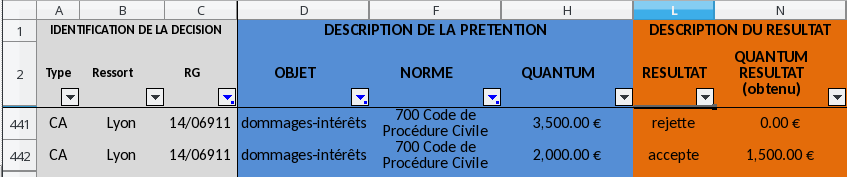
\includegraphics[width=\textwidth]{tab-annotations.png}
\caption{Structure du tableau d'annotations manuelles à remplir: les noms des champs sont sur les 2 premières lignes et les demandes sont données en exemple pour la catégorie \textit{dommages-intérêts sur le fondement de l'article 700 du code de procédure civile} (décision 14/06911 de la cour d'appel de Lyon).} \label{tab:quanta:tab-annotations}
\end{table}

Le problème est ainsi décomposé grossièrement en 3 tâches:
\begin{enumerate}
\item identification des catégories présentes dans le document pour n'appliquer l'extraction  que de ces catégories;
\item identification des attributs des demandes de chaque catégorie détectée: quanta demandés, quantas obtenus, et sens du résultat;
\item résolution des coréférences: Liaison des données relatives à la même demande
\end{enumerate}

 Dans la section suivante, nous synthétisons l'analogie avec des problématiques couramment traités et explorons les approches proposées dans des travaux publiés.

\section{Synthèse bibliographique associée}
\label{sec:quanta:biblio}
Chacune de ses tâches se rapproche d'une tâche traitée dans la litérature, et nous donne ainsi des voies de solution. En effet, la détection de catégories dans les décisions peut être modélisée comme un problème de classification de document. Les deux dernières tâches se rapprochent plus de problématiques d'extraction d'entités complexes à champs/attributs comme l'extraction d'évènements, le remplissage de champs, ou encore l'extraction d'entités ou de rôles sémantiques et la résolution de coréférencement.

\subsection{Analogie avec des problématiques de la litératures}
\begin{itemize}
\item Extraction d'évènement : 
\end{itemize}
\begin{table}[h]
\small
\begin{tabular}{|p{0.13\textwidth}|p{0.3\textwidth}|p{0.4\textwidth}|}
\hline
\textbf{Champs} & \textbf{\cite{ace2005event}} & \textbf{Analogie chez les demandes} \\ \hline
\textbf{Type} &  Die & Catégorie="Dommages-intérêts pour procédure abusive" \\ \hline
\textbf{Expression} (\textit{extend}) & "Il est \textbf{mort} hier d'une insuffisance rénale."  & (\textit{voir page précédente}) \\ \hline
\textbf{Déclencheur} & "mort" & "procédure abusive"\\ \hline
\textbf{Argument} & Victim-Arg="il" \linebreak Time-Arg="hier"  & Quantum-demandé="3000\euro{}"\linebreak  Quantum-obtenu="0 \euro{}"\ \\ \hline
\textbf{Attribut} & Polarity=POSITIVE, Tense=PAST & Sens-résultat="Rejeté" \\ \hline
\end{tabular}
\caption{Exemple d'analogie entre les évènements et l'extraction de demande}
\end{table}
\begin{itemize}
\item Remplissage de champs des entités \textbf{Demande} (\textit{slot-filling)}: \textbf{Catégorie, Quantum-demandé, Quantum-obtenu, Sens-résultat}
\item Extraction d'entités et relations ou résolution de coréférence: par ex. \textbf{(quantum demandé, quantum obtenu)}
\end{itemize}

\subsection{Approches}
\begin{table}[h!]
\small
\begin{tabular}{|p{0.25\textwidth}|p{0.7\textwidth}|}
\hline
\textbf{Type d'approches} & \textbf{Exemples} \\ \hline
\textbf{Chaine de traitement} & \textbf{Chaîne de classifieurs  }\cite{ahn2006stages} \\ \hline
\textbf{Modélisation probabiliste} de la structure de l'évènement & \textbf{Modèle joint d'inférence} des entités, arguments, déclencheurs

$p_\theta(t_i, r_i, a \vert i, N_i, x)$ \cite{yang2016jointEntityEvt} %\linebreak 
\\ \hline
\textbf{Réseau de neuronnes} pour automatiser la génération des caractéristiques et la modélisation de la structure & (i) \textbf{Architecture multicouche de réseaux de neuronnes récurrents}: encodage de la phrase, encodage des contextes, prédiction du déclencheur, prédiction des rôles, mémoire matricielle d'interdépendance déclencheur-argument \cite{nguyen2016jointtrgarg},  

(ii) \textbf{Réseau de pointeur} (\textit{pointer network}): un encodeur de la phrase et des contextes, plusieurs décodeurs (un pour chaque champ) \cite{palm2017e2e-dnn} \\ \hline
\end{tabular}
\caption{Type d'approches}
\end{table}


\section{Méthode1: Localisation à Base d'Expressions clés prédéfinies et Apprises Automatiquement}
\label{sec:quanta:baseline}

\subsection{Sélection des termes clés de la catégories: ngram2vec > cluster de ngram > sélection des clusters associés à la catégorie }

\url{https://github.com/azpoliak/eco}

\section{Méthode2: Chaine d'extraction à base de classification}

\section{Méthode3: Extraction par prédiction structurée}

\section{Expérimentations et interprétation des résultats}
\label{sec:quanta:xp}

\subsection{Annotation de données d'évaluation}
\label{sec:quanta:xp:dataset}
\begin{figure}
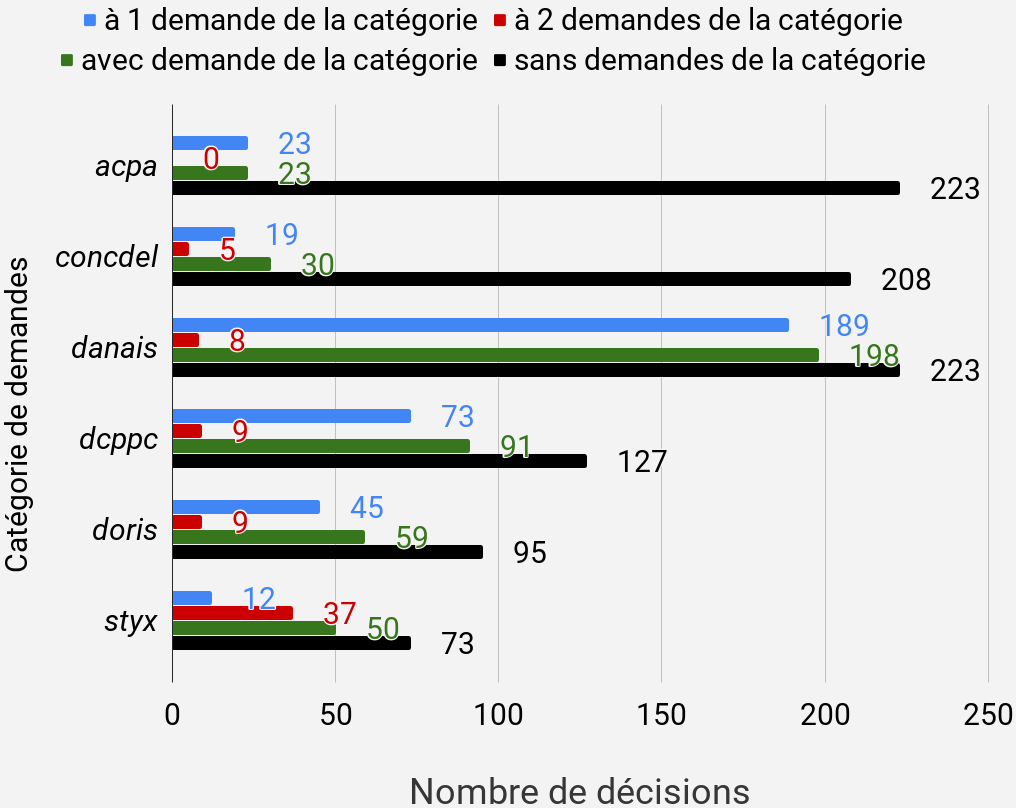
\includegraphics[width=\textwidth]{chartDataset.png}
\caption{Répartitions des demandes dans les documents annotées pour chaque catégorie.}\label{stat-alldata-dmd}
\end{figure}

\subsection{Métriques d'évaluation}
\label{sec:quanta:xp:metrics}
% \begin{figure}[htb]
% 	\includegraphics[width=\textwidth]{gfx/Clean-Thesis-Figure}
% 	\caption{Figure example: \textit{(a)} example part one, \textit{(c)} example part two; \textit{(c)} example part three}
% 	\label{fig:system:example1}
% \end{figure}

\subsection{Cas des décisions à une demande}

\subsection{Cas général}

\section{Conclusion}
\label{sec:quanta:conclusion}

